\chapter{IMPLEMENTATION}
\label{ch:implementation}

This chapter presents the current implementation state of the IU-MiCert system, detailing the development progress across the frontend, CLI tools, and blockchain components. The implementation follows the methodology outlined in Chapter~\ref{ch:methodology} and utilizes the technology stack described in Chapter~\ref{ch:prototyping}. The system is designed to support multiple receipt types including single-term verification and comprehensive academic journey receipts with selective disclosure capabilities.

\section{System Architecture Overview}
\label{sec:architecture_overview}

The IU-MiCert system architecture consists of three primary components working in concert to provide decentralized micro-credential management:

\begin{enumerate}
    \item \textbf{Frontend Client Application}: A React.js-based web interface supporting multiple receipt verification types
    \item \textbf{CLI Tools}: Go-based command-line utilities for Verkle tree construction and credential management
    \item \textbf{Blockchain Infrastructure}: Smart contract-based verification system for on-chain credential validation
\end{enumerate}

The modular design ensures scalability and maintainability while supporting the core functionalities of credential issuance, selective disclosure, and verification as outlined in the system requirements.

\begin{figure}[htbp]
    \centering
    \includegraphics[width=0.8\textwidth]{figures/system_architecture.png}
    \caption{IU-MiCert System Architecture Overview}
    \label{fig:system_architecture}
\end{figure}

\section{Frontend Implementation}
\label{sec:frontend_implementation}

The frontend implementation represents the most mature component of the IU-MiCert system, providing a comprehensive user interface for credential verification and receipt management.

\subsection{Client Application Architecture}
\label{subsec:client_architecture}

The client application is built using React.js with Next.js framework, leveraging TypeScript for type safety and enhanced developer experience. The application architecture follows a component-based design pattern, ensuring modularity and reusability across different verification workflows.

\subsubsection{Receipt Type Support}
The frontend application supports multiple receipt verification types to accommodate various credential scenarios:

\begin{itemize}
    \item \textbf{Single Term Receipts}: Verification of credentials for a specific academic term or period
    \item \textbf{Academic Journey Receipts}: Comprehensive verification of multiple terms representing complete academic progression
    \item \textbf{Selective Disclosure}: Granular control over which credentials are revealed during verification
\end{itemize}

The implementation utilizes a unified interface that dynamically adapts based on the receipt type, providing optimal user experience while maintaining consistency across different verification scenarios.

\subsubsection{Verification Workflow Implementation}
The verification workflow implementation handles the complete process from receipt upload to credential validation:

\begin{enumerate}
    \item \textbf{Receipt Upload}: Secure handling of journey receipts with format validation
    \item \textbf{Proof Parsing}: Extraction and validation of Verkle proofs from receipt data
    \item \textbf{Blockchain Interaction}: Communication with smart contracts for root commitment verification
    \item \textbf{Result Display}: Comprehensive presentation of verification results with detailed credential information
\end{enumerate}

The implementation ensures that all verification steps are performed securely and efficiently, with appropriate error handling and user feedback throughout the process.

\subsection{User Interface Components}
\label{subsec:ui_components}

The frontend implementation includes several key UI components designed for optimal user experience across different verification workflows. The system provides specialized interfaces for each receipt type, ensuring users can efficiently navigate through various credential verification scenarios.

\begin{figure}[htbp]
    \centering
    \includegraphics[width=1\textwidth]{figures/landing-ui.png}
    \caption{Client Site Landing - \url{https://iu-micert.vercel.app/}}
    \label{fig:verify-ui}
\end{figure}

\subsubsection{Main Verification Interface}
The primary entry point for all verification activities provides a unified starting interface:

\begin{figure}[htbp]
    \centering
    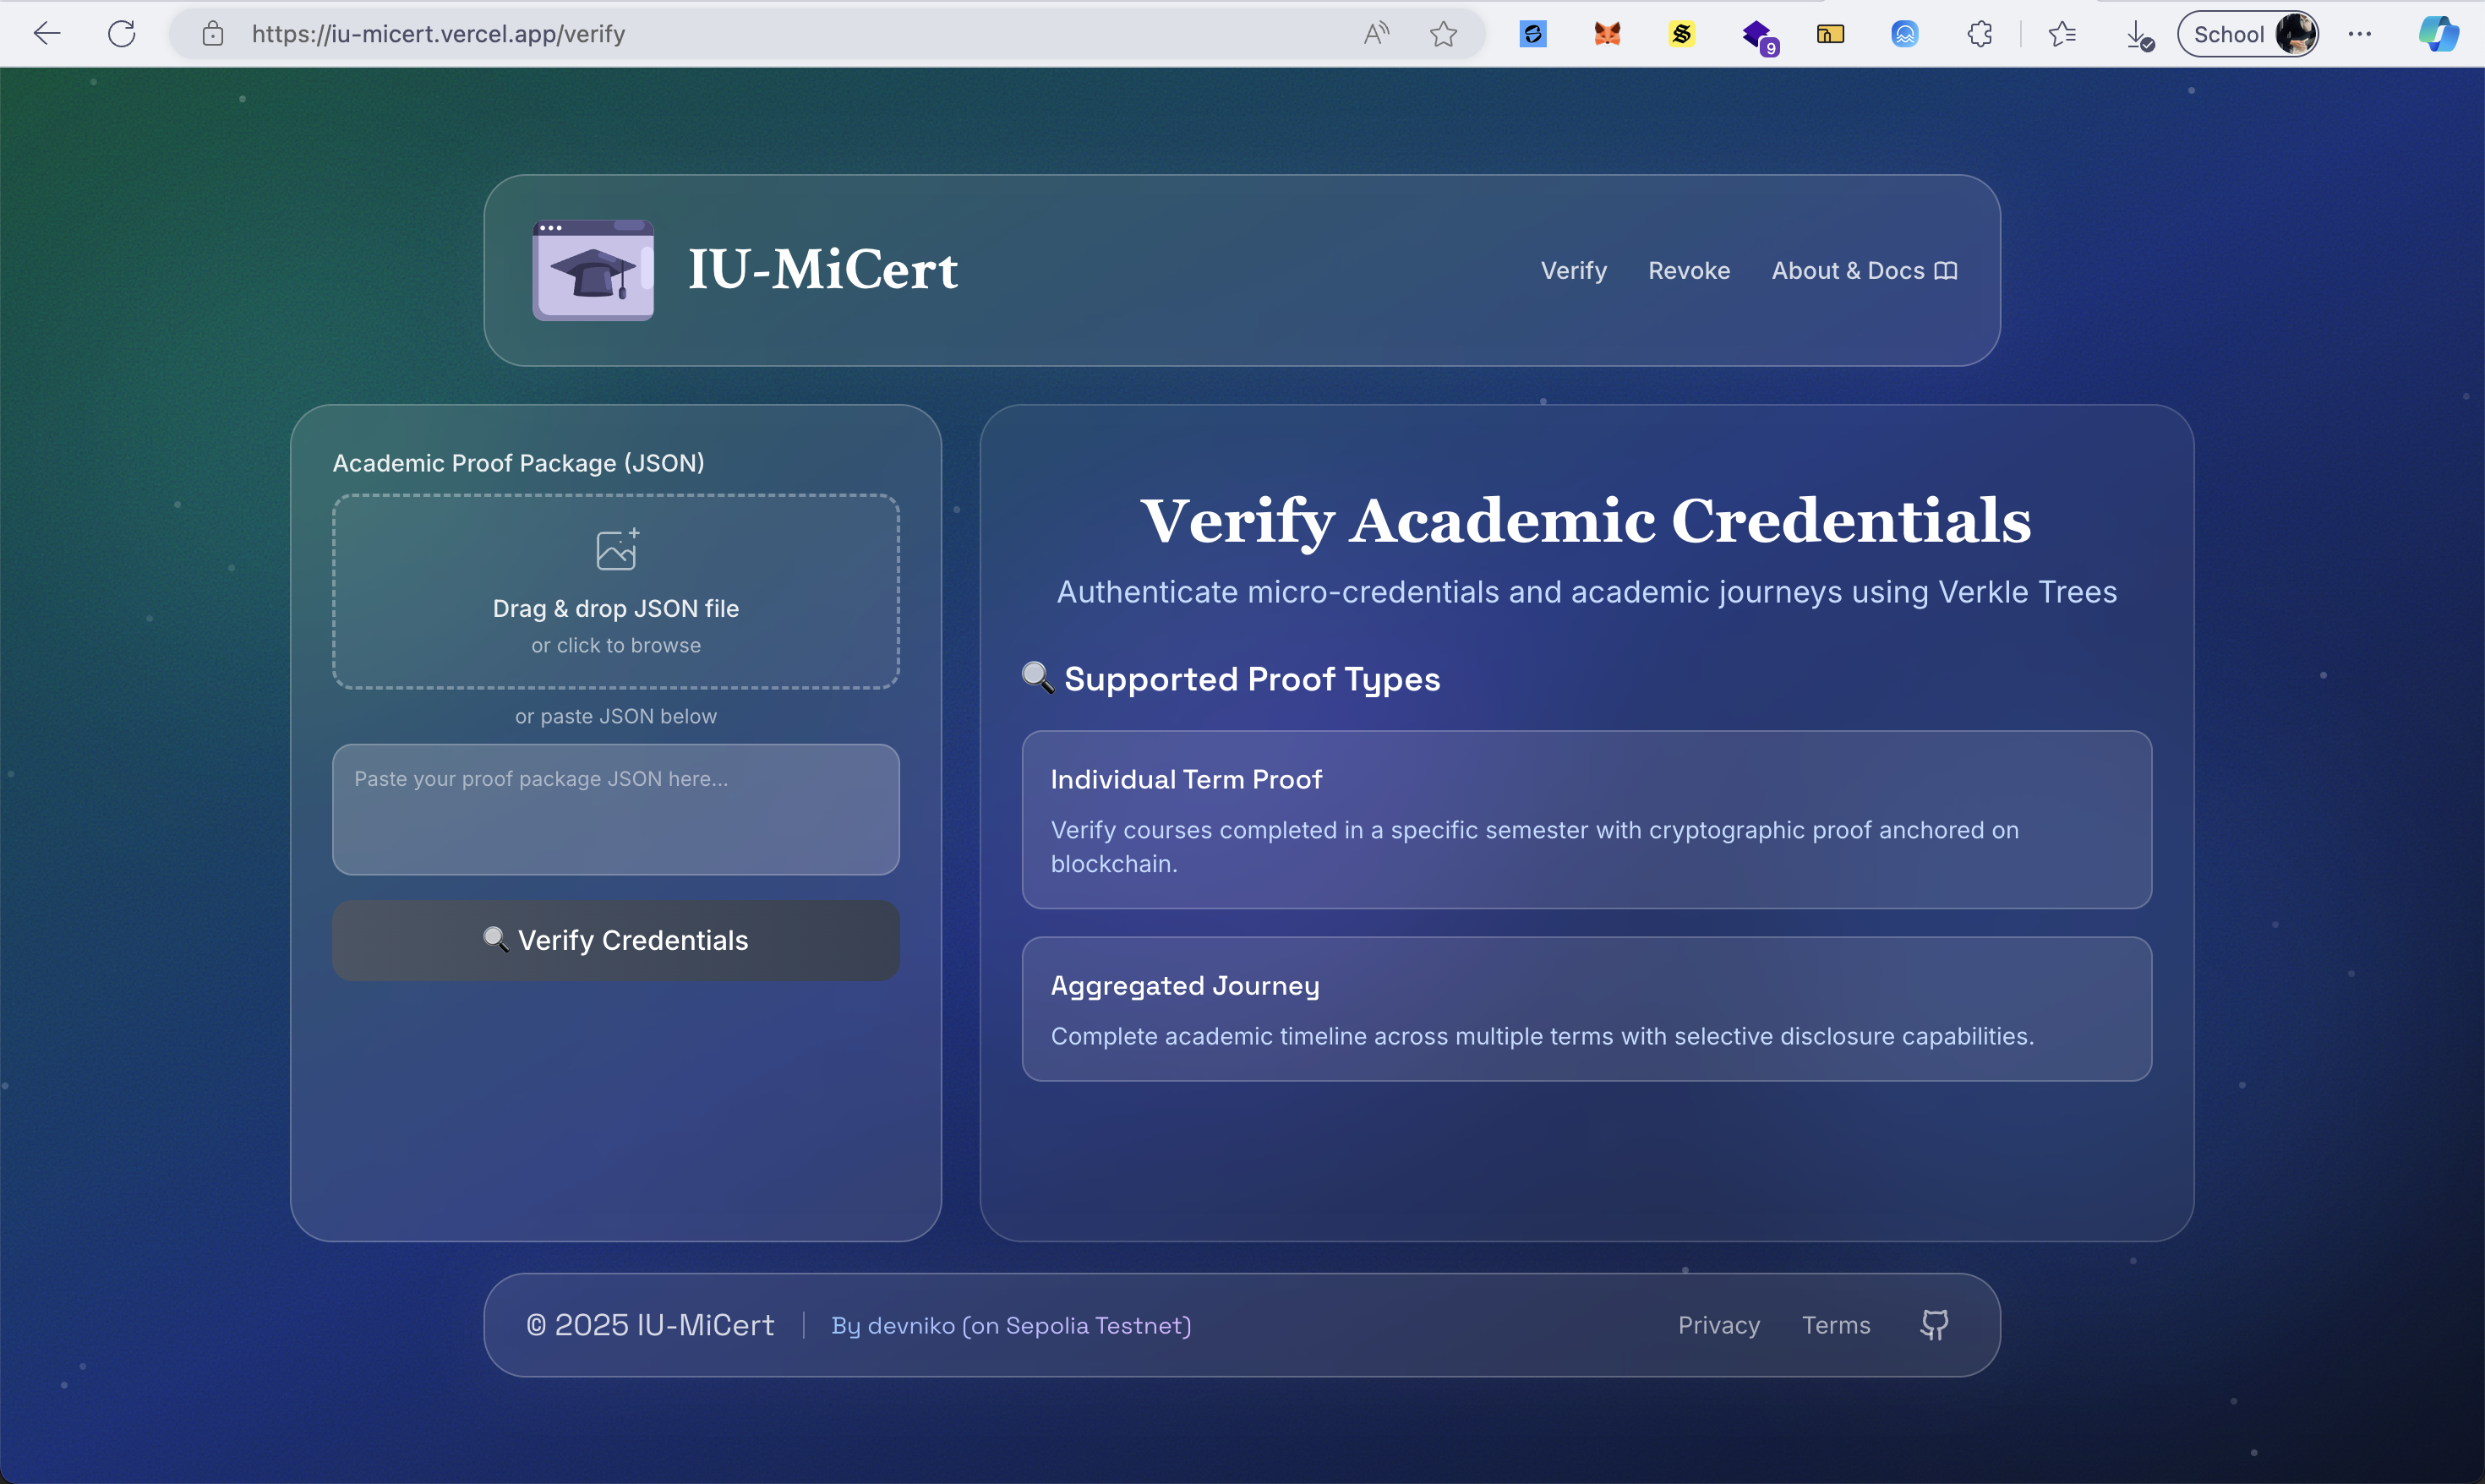
\includegraphics[width=1\textwidth]{figures/verify-ui.png}
    \caption{Main Verification Interface - Entry Point for All Receipt Types}
    \label{fig:verify-ui}
\end{figure}

The main verification interface (Figure~\ref{fig:verify-ui}) offers:
\begin{itemize}
    \item Intuitive receipt type selection
    \item Drag-and-drop upload functionality with format validation
    \item Clear workflow guidance for different verification scenarios
    \item Responsive design ensuring optimal display across all devices
\end{itemize}

\subsubsection{Single Term Verification Interface}
For focused credential verification of specific academic periods:

\begin{figure}[htbp]
    \centering
    \includegraphics[width=1\textwidth]{figures/term-verify.png}
    \caption{Single Term Verification Interface}
    \label{fig:term-verify}
\end{figure}

The single term interface (Figure~\ref{fig:term-verify}) provides:
\begin{itemize}
    \item Streamlined workflow for individual term verification
    \item Detailed credential display with comprehensive metadata
    \item Real-time verification progress indicators
\end{itemize}

\subsubsection{Academic Journey Verification Interface}
For comprehensive multi-term credential verification:

\begin{figure}[htbp]
    \centering
    \includegraphics[width=1\textwidth]{figures/journey-verify.png}
    \caption{Academic Journey Verification Interface}
    \label{fig:journey-verify}
\end{figure}

The journey verification interface (Figure~\ref{fig:journey-verify}) features:
\begin{itemize}
    \item Multi-term credential organization and display
    \item Timeline visualization for academic progression
    \item Batch verification capabilities with individual term status
    \item Comprehensive academic history presentation
\end{itemize}

\subsubsection{Academic Journey Lookup}
For advanced journey receipt management with lookup capabilities:

\begin{figure}[htbp]
    \centering
    \includegraphics[width=1\textwidth]{figures/journey-lookup-verify.png}
    \caption{Journey Lookup}
    \label{fig:journey-lookup-verify}
\end{figure}

The journey lookup interface (Figure~\ref{fig:journey-lookup-verify}) delivers:
\begin{itemize}
    \item Quick access to single terms that comprise the journey
\end{itemize}

\subsubsection{Cross-Interface Design Consistency}
All verification interfaces maintain design consistency through:
\begin{itemize}
    \item Unified color scheme and typography across all components
    \item Consistent navigation patterns and user interaction models
    \item Standardized error handling and user feedback mechanisms
    \item Responsive design principles ensuring optimal functionality across desktop, tablet, and mobile devices
\end{itemize}

\subsubsection{Accessibility and Usability Features}
The interface implementation prioritizes accessibility:
\begin{itemize}
    \item WCAG 2.1 compliance for screen reader compatibility
    \item Intuitive user flows with clear progress indicators and helpful guidance text
\end{itemize}

\section{CLI Tools Implementation Status}
\label{sec:cli_implementation}

The CLI tools component represents the next phase of development, building upon existing Verkle tree implementation experience to create comprehensive credential management utilities.

\subsection{Current Development State}
\label{subsec:cli_current_state}

While the CLI tools are not yet fully implemented, the development foundation is well-established based on previous thesis work on single diploma issuance using Verkle tree construction. The existing codebase provides:

\begin{itemize}
    \item Proven Verkle tree construction algorithms
    \item Cryptographic proof generation mechanisms
    \item Secure key management utilities
    \item Blockchain interaction capabilities
\end{itemize}

\subsection{Planned CLI Architecture}
\label{subsec:cli_architecture}

The CLI tools will be implemented in Go, leveraging the \texttt{ethereum/go-verkle} library for cryptographic operations. The planned architecture includes:

\subsubsection{Core Commands}
\begin{itemize}
    \item \texttt{micert init}: Initialize new credential repository
    \item \texttt{micert add-term}: Add new academic term with credentials
    \item \texttt{micert generate-receipt}: Create journey receipts with selective disclosure
    \item \texttt{micert verify-local}: Local verification without blockchain interaction
    \item \texttt{micert publish-roots}: Publish term root commitments to blockchain
\end{itemize}

\subsubsection{Data Format Adaptation}
The CLI implementation will adapt the existing single diploma format to support:
\begin{itemize}
    \item Multi-term credential structures
    \item Hierarchical academic progression
    \item Selective disclosure metadata
    \item Temporal consistency validation
\end{itemize}

\subsection{Implementation Roadmap}
\label{subsec:cli_roadmap}

The CLI development follows a phased approach:

\begin{enumerate}
    \item \textbf{Phase 1}: Adapt existing Verkle tree implementation for multi-term support
    \item \textbf{Phase 2}: Implement journey receipt generation with selective disclosure
    \item \textbf{Phase 3}: Integrate blockchain publishing capabilities
    \item \textbf{Phase 4}: Add comprehensive testing and validation utilities
\end{enumerate}

The implementation leverages proven cryptographic libraries and follows established security practices from the previous diploma issuance system.

% TODO: Add CLI command structure diagram
% \begin{figure}[htbp]
%     \centering
%     \includegraphics[width=0.8\textwidth]{figures/cli_structure.png}
%     \caption{Planned CLI Command Structure}
%     \label{fig:cli_structure}
% \end{figure}

\section{Blockchain Implementation Approach}
\label{sec:blockchain_implementation}

The blockchain component implementation strategy leverages existing verification capabilities while exploring enhanced system architectures for improved efficiency and functionality.

\subsection{Current Blockchain Integration Status}
\label{subsec:blockchain_status}

The blockchain integration is in the planning and design phase, with implementation strategies informed by previous thesis work on on-chain credential verification. The current understanding includes:

\begin{itemize}
    \item Proven feasibility of on-chain Verkle proof verification
    \item Smart contract capabilities for credential validation
    \item Gas optimization strategies for batch operations
    \item Integration patterns with frontend applications
\end{itemize}

\subsection{Implementation Strategies}
\label{subsec:blockchain_strategies}

Two primary approaches are being considered for blockchain implementation:

\subsubsection{Direct Verification Approach}
The direct approach involves:
\begin{itemize}
    \item Individual term verification through separate smart contract calls
    \item Straightforward implementation using existing proof verification functions
    \item Higher gas costs but simpler smart contract logic
    \item Direct compatibility with current frontend verification workflows
\end{itemize}

This approach provides immediate functionality by adapting existing single-term verification to handle multiple terms sequentially.

\subsubsection{Enhanced Batch Verification}
The enhanced approach focuses on:
\begin{itemize}
    \item Batch verification of multiple terms in single transactions
    \item Optimized gas usage through aggregated proof validation
    \item Complex smart contract logic for journey receipt validation
    \item Advanced cryptographic operations for efficient verification
\end{itemize}

This approach requires more sophisticated implementation but offers superior performance and cost-effectiveness for large-scale deployments.

\subsection{Smart Contract Architecture}
\label{subsec:smart_contract_architecture}

The planned smart contract architecture builds upon the pseudocode outlined in Chapter \ref{ch:methodology} (Methodology), extending functionality to support:

\subsubsection{Enhanced Storage Management}
\begin{itemize}
    \item Hierarchical term organization by academic periods
    \item Efficient root commitment storage with metadata
    \item Revocation management with granular control
    \item Access control for authorized credential issuers
\end{itemize}

\subsubsection{Advanced Verification Functions}
\begin{itemize}
    \item Batch verification capabilities for journey receipts
    \item Temporal consistency validation across multiple terms
    \item Academic progression rule enforcement
    \item Selective disclosure support with privacy preservation
\end{itemize}

\subsection{Development Priorities}
\label{subsec:blockchain_priorities}

The blockchain implementation prioritizes:

\begin{enumerate}
    \item \textbf{Security}: Comprehensive cryptographic validation and access control
    \item \textbf{Efficiency}: Gas-optimized operations for cost-effective verification
    \item \textbf{Compatibility}: Seamless integration with existing frontend and CLI components
    \item \textbf{Scalability}: Architecture supporting high-volume credential verification
\end{enumerate}

The implementation will begin with the direct verification approach to establish baseline functionality, followed by enhancement to batch verification for improved performance.

% TODO: Add blockchain interaction flow diagram
% \begin{figure}[htbp]
%     \centering
%     \includegraphics[width=0.8\textwidth]{figures/blockchain_flow.png}
%     \caption{Blockchain Verification Workflow}
%     \label{fig:blockchain_flow}
% \end{figure}

\section{Integration and Testing Strategy}
\label{sec:integration_testing}

The implementation strategy emphasizes thorough integration testing and validation across all system components to ensure reliable operation and security.

\subsection{Component Integration}
\label{subsec:component_integration}

The integration approach follows a systematic methodology:

\begin{enumerate}
    \item \textbf{Frontend-CLI Integration}: Ensuring seamless data flow between web interface and command-line tools
    \item \textbf{CLI-Blockchain Integration}: Validating smart contract interactions and transaction handling
    \item \textbf{End-to-End Workflows}: Complete credential lifecycle testing from issuance to verification
    \item \textbf{Cross-Component Validation}: Ensuring data consistency and format compatibility
\end{enumerate}

\subsection{Testing Framework}
\label{subsec:testing_framework}

The testing strategy encompasses:

\subsubsection{Unit Testing}
\begin{itemize}
    \item Individual component functionality validation
    \item Cryptographic operation correctness verification
    \item Data format and serialization testing
    \item Error handling and edge case coverage
\end{itemize}

\subsubsection{Integration Testing}
\begin{itemize}
    \item Cross-component communication validation
    \item Blockchain transaction testing on Sepolia testnet
    \item Performance benchmarking for large credential sets
    \item Security audit of cryptographic implementations
\end{itemize}

\subsubsection{User Acceptance Testing}
\begin{itemize}
    \item Realistic workflow simulation with generated test data
    \item User interface usability evaluation
    \item Performance testing under various load conditions
    \item Compatibility testing across different browser environments
\end{itemize}

\section{Current Limitations and Future Enhancements}
\label{sec:limitations_enhancements}

The current implementation state presents several limitations that will be addressed in future development phases:

\subsection{Current Limitations}
\label{subsec:current_limitations}

\begin{itemize}
    \item \textbf{CLI Tools}: Not yet implemented, limiting end-to-end credential management capabilities
    \item \textbf{Blockchain Integration}: Pending implementation of smart contract verification system
    \item \textbf{Scalability Testing}: Limited validation with large-scale credential datasets
    \item \textbf{Production Deployment}: Current implementation focused on development and testing environments
\end{itemize}

\subsection{Planned Enhancements}
\label{subsec:planned_enhancements}

Future development will address current limitations through:

\begin{itemize}
    \item \textbf{Complete CLI Implementation}: Full command-line utility suite for credential management
    \item \textbf{Advanced Blockchain Features}: Enhanced smart contract capabilities with batch verification
    \item \textbf{Performance Optimization}: Improved efficiency for large-scale credential processing
    \item \textbf{Security Auditing}: Comprehensive security analysis and vulnerability assessment
    \item \textbf{Production Readiness}: Deployment optimization and monitoring capabilities
\end{itemize}

\section{Chapter Summary}
\label{sec:implementation_summary}

This chapter has presented the current implementation state of the IU-MiCert system, highlighting the completed frontend components, planned CLI tools development, and blockchain integration strategy. The implementation demonstrates significant progress in creating a comprehensive decentralized credential management system with advanced privacy features.

The frontend implementation provides a robust foundation for credential verification and receipt management, supporting multiple verification types and selective disclosure capabilities. The planned CLI tools development builds upon proven Verkle tree implementation experience, while the blockchain integration strategy balances immediate functionality with long-term performance optimization.

The systematic approach to implementation ensures that each component contributes effectively to the overall system architecture while maintaining security, efficiency, and user experience standards. The integration and testing strategy provides confidence in system reliability and prepares for future enhancements and production deployment.

The current progress establishes a solid foundation for the complete IU-MiCert system implementation, with clear development paths for the remaining components and a comprehensive understanding of the technical challenges and solutions involved in decentralized credential management.